% !TEX program = lualatex
% !TEX encoding = UTF-8
\documentclass[paper=a4, fontsize=11pt]{jlreq}

% 必要なパッケージの読み込み
\usepackage{luatexja}
\usepackage{graphicx}
\usepackage{booktabs}
\usepackage{tabularx}
\usepackage{hyperref}
\usepackage{tikz}
\usepackage{float}
\usetikzlibrary{shapes.geometric, arrows, positioning, fit, backgrounds}

\title{SportEase の情報の取り扱い}
\author{佐藤佑作} % 必要に応じて記入してください
\date{\today}

\begin{document}

\maketitle

\section{個人情報保護方針}

本システムにおける個人情報の取り扱いは、以下の通り厳格に管理する。

\subsection{Google認証で収集する個人情報}
利用するGoogleアカウントから取得する個人情報はメールアドレスのみである。

メールアドレスは本システム内でユーザーを一意に識別するIDとして使用する。

\subsection{データの保存期間と表示}
\begin{itemize}
    \item \textbf{保存期間}: 過去のイベント結果(トーナメント表、順位、得点等)は、学校行事の記録として永続的に保存する。
    \item \textbf{表示ポリシー}:
    \begin{itemize}
        \item 現在進行中のイベントについては、ユーザー名(表示名)を表示する。
        \item 終了した過去のイベントについては、プライバシー保護のためユーザー名を非表示とし、クラス単位またはチーム単位の結果のみを表示する。
        \item 卒業生の個人データ(メールアドレス等)はホワイトリストから削除されるため、システムへのログインは不可能となる。
    \end{itemize}
\end{itemize}

\subsection{アクセス制御}
データベースへのアクセスは以下の通り厳密に制限する。
\begin{itemize}
    \item \textbf{Root (システム管理者)}: 全データへのアクセス権限を持つ。
    \item \textbf{Admin (行事委員)}: 運営に必要な最小限のデータ(試合結果、出欠状況)のみ参照・更新可能。
    \item \textbf{Student (一般学生)}: 自身のプロフィールおよび公開された競技結果のみ閲覧可能。他者のメールアドレス等は閲覧不可。
    \item \textbf{DB直接アクセス(システム外からのアクセス)}: 定められたシステム管理者(1〜2名)のみが、SSH接続を通してのみアクセス可能。
\end{itemize}

\subsection{情報の使用用途}
\begin{table}[H]
    \centering
    \caption{情報の使用用途}
    \begin{tabularx}{\textwidth}{|l|X|}
        \toprule
        情報 & 用途 \\
        \midrule
        メールアドレス & ユーザー認証(OAuth2)、システムからの重要なお知らせ(Web Push通知) \\
        クラス・学年 & トーナメントのチーム分け、クラス対抗戦の集計 \\
        \bottomrule
    \end{tabularx}
\end{table}

\newpage

ユーザーの表示名に関しては、初回ログイン時に以下の画面で設定し、その後自由に変更可能にできる 。
\begin{figure}[htbp]
  \centering
  \includegraphics[width=0.8\linewidth]{./first-login.png}
  \caption{初回ログイン時の表示}
  \label{fig:image}
\end{figure}


\newpage

\section{外部設計}

\subsection{ユーザーロール}
本システムでは以下の3つのベースロールを定義し、権限管理を行っている。\\
必要に応じてロールを増やすことはできるが、権限管理はこの3つのベースロールで行っている。
なお、チーム管理機能に限り、class\_rep(クラス代表)ロールが追加で使用される。

\begin{table}[H]
    \centering
    \caption{ユーザーロール一覧}
    \begin{tabularx}{\textwidth}{|l| X|}
        \toprule
        ロール名 & 概要 \\
        \midrule
        Student (一般学生) & 主に情報の閲覧(対戦表、試合結果、クラスの進捗)および通知の受信を行う。  \\ \midrule
        Admin (行事委員) & イベント全体の管理、試合結果の入力・承認、スケジュールの変更、MVP投票の管理など、運営に必要な全機能にアクセス可能。 \\ \midrule
        Root (システム管理者) & システム設定、ホワイトリスト管理、マスターデータ(スポーツ、クラス等)の管理を行う最高権限。 \\
        \bottomrule
    \end{tabularx}
\end{table}

Roleの制限について、上記のいずれかのロール+class\_repの権限を持つことができる。\\
また、必要に応じて審判等の特定の集団用のロールを作成することも可能である。\\
ベースロールに加えて作成してロールは主に通知機能のロールフィルタリングで用いることを想定している。

\subsection{機能要件}
各ロールにおける利用可能な機能の詳細は以下の通りである。

\subsubsection{Student (一般学生)}
一般的な学生ユーザーに割り当てられるロールであり、以下の機能を利用可能である。
\begin{itemize}
    \item \textbf{アカウント管理}:
    \begin{itemize}
        \item Googleアカウントを用いたログイン・ログアウト
        \item プロフィール設定(表示名、所属クラスの登録)
    \end{itemize}
    \item \textbf{情報閲覧}:
    \begin{itemize}
        \item 開催中のイベント情報の閲覧
        \item 各競技のトーナメント表・対戦組み合わせの閲覧
        \item 試合結果および勝敗のリアルタイム確認
        \item クラス別の総合得点・進捗状況・順位の閲覧
        \item 昼企画(リレー・綱引き等)の結果閲覧
    \end{itemize}
    \item \textbf{チーム管理(自クラスのみ)}:
    \begin{itemize}
        \item 所属クラスのチームメンバー編成機能(メンバーの追加・削除)
        \item チームメンバーの確認
    \end{itemize}
    \item \textbf{通知・その他}:
    \begin{itemize}
        \item 試合開始・結果等のWeb Push通知の受信
        \item MVP投票への参加(投票権がある場合)
    \end{itemize}
\end{itemize}

\subsubsection{Admin (行事委員)}
イベント運営の実務を担当するロールであり、Studentの全機能に加え、以下の管理機能を利用可能である。
\begin{itemize}
    \item \textbf{試合進行管理}:
    \begin{itemize}
        \item 試合開始時間の変更・調整
        \item 試合結果(スコア・勝者)の入力・確定
        \item 試合ステータスの更新(試合中、終了など)
        \item 昼企画(リレー・綱引き等)の予選・決勝結果の入力
    \end{itemize}
    \item \textbf{運営管理}:
    \begin{itemize}
        \item 前日・当日の出欠確認・登録
        \item 各競技の参加定員数の調整・変更
        \item ユーザーの表示名修正(不適切な名前の修正等)
        \item 運営用画像・PDF資料(要項・ルールブック等)のアップロード
        \item MVP投票状況の確認・集計
        \item 行事委員権限の付与・剥奪
    \end{itemize}
\end{itemize}

\subsubsection{Root (システム管理者)}
システムの全権限を持つロールであり、マスターデータの管理を含む以下の高度な機能を利用可能である。
\begin{itemize}
    \item \textbf{システム・イベント設定}:
    \begin{itemize}
        \item ログイン許可リスト(ホワイトリスト)の管理(追加・削除・一括インポート)
        \item 新規イベントの作成およびアクティブイベントの切り替え
        \item 雨天モード(スケジュール短縮・変更時)の切り替えおよび設定管理
    \end{itemize}
    \item \textbf{マスターデータ管理}:
    \begin{itemize}
        \item 競技種目の新規作成・削除
        \item クラス情報の管理および在籍学生数の登録(CSVインポート対応)
        \item 昼企画のグループ分け・テンプレート管理
        \item 全競技のトーナメント表の一括自動生成・プレビュー
    \end{itemize}
    \item \textbf{全体通知}:
    \begin{itemize}
        \item 全ユーザーまたは特定のロールに向けた任意のお知らせ通知の配信
    \end{itemize}
\end{itemize}

\subsection{画面構成・遷移}
本システムはWebブラウザ上で動作するSSR/CSRハイブリッド構成のWebアプリケーション(SvelteKit + adapter-node)であり、以下の画面構成を持つ。

\begin{itemize}
    \item \textbf{ログイン画面}: Googleアカウントによる認証エントリポイント。
    \item \textbf{ダッシュボード (ホーム)}: ログイン後の初期画面。ユーザーロールに応じたメニューを表示。
    \item \textbf{学生向けメニュー (Student)}:
    \begin{itemize}
        \item \textbf{マイページ}: プロフィール設定、クラス情報確認
        \item \textbf{競技・イベント情報}: トーナメント表閲覧、競技詳細、点数一覧
        \item \textbf{昼企画}: 昼競技の結果確認
        \item \textbf{その他}: QRコード表示、通知確認、通知申請
    \end{itemize}
    \item \textbf{運営管理者メニュー (Admin)}:
    \begin{itemize}
        \item \textbf{試合管理}: 試合結果入力、トーナメント進行管理、昼競技結果入力
        \item \textbf{参加管理}: クラス・チーム編成管理、QRコード読み取り・参加確認、出席登録
        \item \textbf{運営設定}: ロール管理、競技詳細設定、MVP投票管理
    \end{itemize}
    \item \textbf{システム管理者メニュー (Root)}:
    \begin{itemize}
        \item \textbf{マスター管理}: イベント作成、競技種目設定、ホワイトリスト管理
        \item \textbf{全体設定}: 雨天モード設定、トーナメント一括生成、クラス人数設定
        \item \textbf{コンテンツ管理}: 競技要項アップロード、MVP確認
    \end{itemize}
\end{itemize}

\subsection{動作環境}
\begin{itemize}
    \item \textbf{クライアント端末}: スマートフォン(iOS/Android)、タブレット、PC
    \item \textbf{推奨ブラウザ}: Google Chrome, Safari, Microsoft Edge (各最新版)
    \item \textbf{ネットワーク}: インターネット接続必須(学内Wi-Fiまたはモバイルネットワーク)
\end{itemize}

\subsection{セキュリティ対策}
本システムでは、以下の多層的なセキュリティ対策を実装している。

\subsubsection{アプリケーションセキュリティ}
\begin{itemize}
    \item \textbf{SQLインジェクション対策}: すべてのデータベース操作において、Go言語のプレースホルダ機能(Prepared Statements)を使用し、SQLインジェクションを無効化している。
    \item \textbf{CSRF対策}: セッションベースの認証(SameSite=Lax Cookie)およびCORSによるOrigin検証により、不正なクロスサイトリクエストを防止している。
    \item \textbf{XSS対策}: SvelteKitのオートエスケープ機能により、ユーザー入力のスクリプト実行を防止している。Markdown表示箇所については、isomorphic-dompurifyによるサニタイズ処理を行っている。
    \item \textbf{API認可}: 各エンドポイントにおいてミドルウェア(Middleware)による認証・認可チェックを行い、権限のないリソースへのアクセスを遮断している。一部の公開エンドポイント(クラス一覧取得、WebSocket接続)は認証不要でアクセス可能。
    \item \textbf{ファイルアップロード}: 画像およびPDFファイルのアップロード時は、拡張子だけでなくMIMEタイプの検証(\texttt{http.DetectContentType})を行い、実行可能ファイルの混入を防ぐ。
\end{itemize}

\subsubsection{インフラストラクチャ・通信}
\begin{itemize}
    \item \textbf{通信の暗号化}: Let's Encryptを用いたSSL/TLS証明書の自動更新により、全通信をHTTPS化している。
    \item \textbf{ポート制限}: 本番環境では外部(インターネット)にはHTTP(80)とHTTPS(443)のみを公開し、DBポート(3306)やSSHポートは外部から遮断している。
    \item \textbf{コンテナ隔離}: Dockerによりアプリケーションとホスト環境を分離し、コンテナ侵害時の影響を最小限に抑えている。
\end{itemize}

\subsection{運用管理規定}

\subsubsection{管理体制}
\begin{itemize}
    \item \textbf{運用責任者}: 行事委員会
    \item \textbf{システム管理者}: 佐藤佑作
    \item \textbf{サーバー管理者}: 林航平、佐藤佑作
\end{itemize}

\subsubsection{引継ぎ}
\begin{itemize}
    \item \textbf{卒業時の処理}: システム管理者が卒業する際は、アクセス権限(サーバーログイン情報、DBパスワード)を変更し、新管理者へ安全に引き継ぐ。旧管理者のアカウントは即座に無効化する。
\end{itemize}

\section{内部設計}

\subsection{システムアーキテクチャ}
本システムはDockerコンテナを用いたマイクロサービス構成を採用している。

\begin{itemize}
    \item \textbf{Reverse Proxy (Traefik)}: エントリーポイントとしてHTTPS通信の終端、Let's EncryptによるSSL証明書の自動更新、およびFrontend/Backendへのルーティングを行う。
    \item \textbf{Frontend (Frontapp)}: SvelteKit (Node.js) を用いたSSR/CSRハイブリッド構成。ユーザーインターフェースを提供。
    \item \textbf{Backend (Backapp)}: Go言語 (Gin Framework) によるREST APIサーバー。ビジネスロジックおよびWebSocketによるリアルタイム配信を担当。
    \item \textbf{Database (DB)}: MySQL 8.0。永続化データを管理。
\end{itemize}

\subsection{技術スタック}
\begin{table}[H]
    \centering
    \caption{採用技術一覧}
    \begin{tabularx}{\textwidth}{l l}
        \toprule
        カテゴリ & 技術 \\
        \midrule
        フロントエンド & SvelteKit, TailwindCSS, TypeScript \\
        バックエンド & Go 1.24, Gin, Gorilla WebSocket \\
        データベース & MySQL 8.0 \\
        インフラ & Docker, Docker Compose, Traefik v2 \\
        認証 & Google OAuth2 (OpenID Connect) \\
        \bottomrule
    \end{tabularx}
\end{table}

\subsection{データモデル設計}
主なエンティティとその役割は以下の通りである。

\begin{itemize}
    \item \textbf{Users}: ユーザーID、メールアドレス、ロール、表示名を管理。
    \item \textbf{Events}: 球技大会等のイベント単位。アクティブなイベントは別テーブル(active\_event)で管理。
    \item \textbf{Sports / Classes}: 競技種目および参加クラスのマスターデータ。
    \item \textbf{Teams / Entries}: クラス・競技ごとのチーム編成およびエントリー情報。
    \item \textbf{Tournaments / Matches}: トーナメント構造および個々の試合データ(開始時刻、スコア、勝者)。
    \item \textbf{Noon Games}: 昼企画のセッション、試合、結果、ポイント、テンプレート実行を管理。
    \item \textbf{Notifications}: Web Push通知の購読情報、通知履歴、および通知リクエストのワークフローを管理。
\end{itemize}

\subsection{データベース設計}
詳細なデータベース設計は以下の通りである。データベースは全35テーブルで構成される。
ここでは主要なテーブルを記載する。

\subsubsection{Core Tables}
基本となるユーザー、イベント、競技、クラス等のテーブル群。

\begin{table}[H]
    \centering
    \caption{users (ユーザー)}
    \begin{tabularx}{\textwidth}{|l|l|X|}
        \toprule
        Column & Type & Description \\
        \midrule
        id & CHAR(36) & UUID (Primary Key) \\
        email & VARCHAR(255) & メールアドレス (Unique) \\
        display\_name & VARCHAR(255) & 表示名 \\
        class\_id & INT & 所属クラスID (FK) \\
        is\_profile\_complete & BOOLEAN & プロフィール登録完了フラグ \\
        created\_at & TIMESTAMP & 作成日時 \\
        updated\_at & TIMESTAMP & 更新日時 \\
        \bottomrule
    \end{tabularx}
\end{table}

\begin{table}[H]
    \centering
    \caption{roles (ロールマスタ)}
    \begin{tabularx}{\textwidth}{|l|l|X|}
        \toprule
        Column & Type & Description \\
        \midrule
        id & INT & Primary Key \\
        name & VARCHAR(50) & ロール名 (root, admin, student) \\
        \bottomrule
    \end{tabularx}
\end{table}

\begin{table}[H]
    \centering
    \caption{user\_roles (ユーザーロール割り当て)}
    \begin{tabularx}{\textwidth}{|l|l|X|}
        \toprule
        Column & Type & Description \\
        \midrule
        user\_id & CHAR(36) & ユーザーID (FK) \\
        role\_id & INT & ロールID (FK) \\
        event\_id & INT & イベントID (FK, NULLable) \\
        \bottomrule
    \end{tabularx}
\end{table}

\begin{table}[H]
    \centering
    \caption{events (イベント・大会)}
    \begin{tabularx}{\textwidth}{|l|l|X|}
        \toprule
        Column & Type & Description \\
        \midrule
        id & INT & Primary Key \\
        name & VARCHAR(255) & イベント名 \\
        year & INT & 年度 \\
        season & ENUM & 時期 (spring, autumn) \\
        start\_date & DATE & 開始日 \\
        end\_date & DATE & 終了日 \\
        is\_rainy\_mode & BOOLEAN & 雨天モードフラグ \\
        competition\_guidelines\_pdf\_url & VARCHAR(500) & 競技要項PDF URL \\
        \bottomrule
    \end{tabularx}
\end{table}

\begin{table}[H]
    \centering
    \caption{active\_event (アクティブイベント管理)}
    \begin{tabularx}{\textwidth}{|l|l|X|}
        \toprule
        Column & Type & Description \\
        \midrule
        id & INT & Primary Key \\
        event\_id & INT & イベントID (FK, Unique) \\
        \bottomrule
    \end{tabularx}
\end{table}

\begin{table}[H]
    \centering
    \caption{classes (クラス)}
    \begin{tabularx}{\textwidth}{|l|l|X|}
        \toprule
        Column & Type & Description \\
        \midrule
        id & INT & Primary Key \\
        event\_id & INT & イベントID (FK) \\
        name & VARCHAR(255) & クラス名 \\
        student\_count & INT & 学生数 \\
        attend\_count & INT & 出席数 \\
        \bottomrule
    \end{tabularx}
\end{table}

\begin{table}[H]
    \centering
    \caption{sports (競技マスタ)}
    \begin{tabularx}{\textwidth}{|l|l|X|}
        \toprule
        Column & Type & Description \\
        \midrule
        id & INT & Primary Key \\
        name & VARCHAR(255) & 競技名 \\
        \bottomrule
    \end{tabularx}
\end{table}

\begin{table}[H]
    \centering
    \caption{event\_sports (イベント採用競技)}
    \begin{tabularx}{\textwidth}{|l|l|X|}
        \toprule
        Column & Type & Description \\
        \midrule
        event\_id & INT & イベントID (FK) \\
        sport\_id & INT & 競技ID (FK) \\
        description & TEXT & 説明 \\
        rules & TEXT & ルール \\
        rules\_type & ENUM & ルール形式 (markdown, pdf) \\
        rules\_pdf\_url & VARCHAR(255) & ルールPDF URL \\
        location & ENUM & 場所 (gym1, gym2, ground, noon\_game, other) \\
        min\_capacity & INT & 最少人数 \\
        max\_capacity & INT & 最大人数 \\
        staff\_count & INT & 運営スタッフ数 \\
        \bottomrule
    \end{tabularx}
\end{table}

\begin{table}[H]
    \centering
    \caption{whitelisted\_emails (ログイン許可リスト)}
    \begin{tabularx}{\textwidth}{|l|l|X|}
        \toprule
        Column & Type & Description \\
        \midrule
        email & VARCHAR(255) & メールアドレス \\
        role & ENUM & 初期ロール \\
        event\_id & INT & イベントID (NULLable) \\
        \bottomrule
    \end{tabularx}
\end{table}

\subsubsection{Competition Tables}
トーナメント、試合、チーム、得点等の競技運営に関わるテーブル群。

\begin{table}[H]
    \centering
    \caption{teams (チーム)}
    \begin{tabularx}{\textwidth}{|l|l|X|}
        \toprule
        Column & Type & Description \\
        \midrule
        id & INT & Primary Key \\
        name & VARCHAR(255) & チーム名 \\
        class\_id & INT & クラスID (FK) \\
        sport\_id & INT & 競技ID (FK) \\
        event\_id & INT & イベントID (FK) \\
        min\_capacity & INT & チーム最少人数 \\
        max\_capacity & INT & チーム最大人数 \\
        \bottomrule
    \end{tabularx}
\end{table}

\begin{table}[H]
    \centering
    \caption{team\_members (チームメンバー)}
    \begin{tabularx}{\textwidth}{|l|l|X|}
        \toprule
        Column & Type & Description \\
        \midrule
        team\_id & INT & チームID (FK) \\
        user\_id & CHAR(36) & ユーザーID (FK) \\
        is\_confirmed & BOOLEAN & 参加確定フラグ \\
        \bottomrule
    \end{tabularx}
\end{table}

\begin{table}[H]
    \centering
    \caption{tournaments (トーナメント)}
    \begin{tabularx}{\textwidth}{|l|l|X|}
        \toprule
        Column & Type & Description \\
        \midrule
        id & INT & Primary Key \\
        name & VARCHAR(255) & トーナメント名 \\
        event\_id & INT & イベントID (FK) \\
        sport\_id & INT & 競技ID (FK) \\
        \bottomrule
    \end{tabularx}
\end{table}

\begin{table}[H]
    \centering
    \caption{matches (試合)}
    \begin{tabularx}{\textwidth}{|l|l|X|}
        \toprule
        Column & Type & Description \\
        \midrule
        id & INT & Primary Key \\
        tournament\_id & INT & トーナメントID (FK) \\
        round & INT & ラウンド番号 \\
        match\_number\_in\_round & INT & ラウンド内試合順 \\
        team1\_id & INT & チーム1 ID (FK) \\
        team2\_id & INT & チーム2 ID (FK) \\
        team1\_score & INT & チーム1 スコア \\
        team2\_score & INT & チーム2 スコア \\
        winner\_team\_id & INT & 勝者チームID (FK) \\
        next\_match\_id & INT & 次戦ID (FK) \\
        status & VARCHAR(50) & 試合状態 (scheduled, in\_progress, completed) \\
        start\_time & VARCHAR(255) & 開始予定時刻 \\
        rainy\_mode\_start\_time & VARCHAR(255) & 雨天時開始時刻 \\
        court\_number & VARCHAR(255) & コート番号 \\
        is\_bronze\_match & BOOLEAN & 3位決定戦フラグ \\
        is\_loser\_bracket\_match & BOOLEAN & 敗者復活戦フラグ \\
        loser\_bracket\_round & INT & 敗者復活戦ラウンド \\
        loser\_bracket\_block & VARCHAR(1) & 敗者復活戦ブロック \\
        \bottomrule
    \end{tabularx}
\end{table}

\begin{table}[H]
    \centering
    \caption{class\_scores (クラス得点集計)}
    \begin{tabularx}{\textwidth}{|l|l|X|}
        \toprule
        Column & Type & Description \\
        \midrule
        id & INT & Primary Key \\
        event\_id & INT & イベントID (FK) \\
        class\_id & INT & クラスID (FK) \\
        initial\_points & INT & 初期点 \\
        survey\_points & INT & アンケート点 \\
        attendance\_points & INT & 出席点 \\
        gym1\_win1〜3\_points & INT & 体育館1 勝利点(1〜3勝) \\
        gym1\_champion\_points & INT & 体育館1 優勝点 \\
        gym2\_win1〜3\_points & INT & 体育館2 勝利点(1〜3勝) \\
        gym2\_champion\_points & INT & 体育館2 優勝点 \\
        gym2\_loser\_bracket\_champion\_points & INT & 体育館2 敗者復活戦優勝点 \\
        ground\_win1〜3\_points & INT & グラウンド 勝利点(1〜3勝) \\
        ground\_champion\_points & INT & グラウンド 優勝点 \\
        noon\_game\_points & INT & 昼企画点 \\
        mvp\_points & INT & MVP点 \\
        total\_points\_current\_event & INT & 現イベント得点 \\
        rank\_current\_event & INT & 現イベント順位 \\
        total\_points\_overall & INT & 総合得点 \\
        rank\_overall & INT & 総合順位 \\
        \bottomrule
    \end{tabularx}
\end{table}

\begin{table}[H]
    \centering
    \caption{score\_logs (得点履歴)}
    \begin{tabularx}{\textwidth}{|l|l|X|}
        \toprule
        Column & Type & Description \\
        \midrule
        id & INT & Primary Key \\
        event\_id & INT & イベントID (FK) \\
        class\_id & INT & クラスID (FK) \\
        points & INT & 加算/減算ポイント \\
        reason & TEXT & 理由 \\
        source\_match\_id & INT & 対象試合ID (FK) \\
        created\_at & TIMESTAMP & 作成日時 \\
        \bottomrule
    \end{tabularx}
\end{table}

\begin{table}[H]
    \centering
    \caption{mvp\_votes (MVP投票)}
    \begin{tabularx}{\textwidth}{|l|l|X|}
        \toprule
        Column & Type & Description \\
        \midrule
        id & INT & Primary Key \\
        event\_id & INT & イベントID (FK) \\
        voter\_user\_id & CHAR(36) & 投票者ID (FK) \\
        voted\_for\_class\_id & INT & 被投票クラスID (FK) \\
        reason & TEXT & 理由 \\
        points & INT & 投票ポイント \\
        \bottomrule
    \end{tabularx}
\end{table}

\begin{table}[H]
    \centering
    \caption{check\_ins (チェックイン・出席)}
    \begin{tabularx}{\textwidth}{|l|l|X|}
        \toprule
        Column & Type & Description \\
        \midrule
        id & INT & Primary Key \\
        user\_id & CHAR(36) & ユーザーID (FK) \\
        event\_id & INT & イベントID (FK) \\
        purpose & ENUM & 目的 (opening\_ceremony, event\_participation) \\
        checked\_in\_at & TIMESTAMP & チェックイン日時 \\
        \bottomrule
    \end{tabularx}
\end{table}

\begin{table}[H]
    \centering
    \caption{rainy\_mode\_settings (雨天モード設定)}
    \begin{tabularx}{\textwidth}{|l|l|X|}
        \toprule
        Column & Type & Description \\
        \midrule
        id & INT & Primary Key \\
        event\_id & INT & イベントID (FK) \\
        sport\_id & INT & 競技ID (FK) \\
        class\_id & INT & クラスID (FK) \\
        min\_capacity & INT & 最少人数 \\
        max\_capacity & INT & 最大人数 \\
        match\_start\_time & VARCHAR(255) & 開始時刻 \\
        \bottomrule
    \end{tabularx}
\end{table}

\subsubsection{Noon Game Tables}
昼企画(リレー、綱引き等)に関わるテーブル群。

\begin{table}[H]
    \centering
    \caption{noon\_game\_sessions (昼企画セッション)}
    \begin{tabularx}{\textwidth}{|l|l|X|}
        \toprule
        Column & Type & Description \\
        \midrule
        id & INT & Primary Key \\
        event\_id & INT & イベントID (FK) \\
        name & VARCHAR(255) & 企画名 \\
        description & TEXT & 説明 \\
        mode & ENUM & 対戦モード (class, group, mixed) \\
        win\_points & INT & 勝利ポイント \\
        loss\_points & INT & 敗北ポイント \\
        draw\_points & INT & 引分ポイント \\
        participation\_points & INT & 参加ポイント \\
        allow\_manual\_points & BOOLEAN & 手動ポイント許可フラグ \\
        \bottomrule
    \end{tabularx}
\end{table}

\begin{table}[H]
    \centering
    \caption{noon\_game\_groups (昼企画グループ)}
    \begin{tabularx}{\textwidth}{|l|l|X|}
        \toprule
        Column & Type & Description \\
        \midrule
        id & INT & Primary Key \\
        session\_id & INT & セッションID (FK) \\
        name & VARCHAR(255) & グループ名 (例: 1年合同) \\
        \bottomrule
    \end{tabularx}
\end{table}

\begin{table}[H]
    \centering
    \caption{noon\_game\_group\_members (昼企画グループメンバー)}
    \begin{tabularx}{\textwidth}{|l|l|X|}
        \toprule
        Column & Type & Description \\
        \midrule
        id & INT & Primary Key \\
        group\_id & INT & グループID (FK) \\
        class\_id & INT & クラスID (FK) \\
        weight & DECIMAL(6,2) & 重み係数 \\
        \bottomrule
    \end{tabularx}
\end{table}

\begin{table}[H]
    \centering
    \caption{noon\_game\_matches (昼企画試合)}
    \begin{tabularx}{\textwidth}{|l|l|X|}
        \toprule
        Column & Type & Description \\
        \midrule
        id & INT & Primary Key \\
        session\_id & INT & セッションID (FK) \\
        title & VARCHAR(255) & 試合タイトル \\
        status & ENUM & 状態 (scheduled, in\_progress, completed, cancelled) \\
        home\_side\_type & ENUM & ホーム側種別 (class, group) \\
        home\_class\_id / home\_group\_id & INT & ホーム側ID \\
        away\_side\_type & ENUM & アウェイ側種別 (class, group) \\
        away\_class\_id / away\_group\_id & INT & アウェイ側ID \\
        allow\_draw & BOOLEAN & 引分許可 \\
        \bottomrule
    \end{tabularx}
\end{table}

\begin{table}[H]
    \centering
    \caption{noon\_game\_results (昼企画試合結果)}
    \begin{tabularx}{\textwidth}{|l|l|X|}
        \toprule
        Column & Type & Description \\
        \midrule
        id & INT & Primary Key \\
        match\_id & INT & 試合ID (FK, Unique) \\
        winner & ENUM & 勝者 (home, away, draw) \\
        home\_score & INT & ホーム側スコア \\
        away\_score & INT & アウェイ側スコア \\
        recorded\_by & CHAR(36) & 記録者ID (FK) \\
        \bottomrule
    \end{tabularx}
\end{table}

\begin{table}[H]
    \centering
    \caption{noon\_game\_template\_runs (テンプレート実行)}
    \begin{tabularx}{\textwidth}{|l|l|X|}
        \toprule
        Column & Type & Description \\
        \midrule
        id & INT & Primary Key \\
        session\_id & INT & セッションID (FK) \\
        template\_key & VARCHAR(50) & テンプレート識別子 (year\_relay等) \\
        name & VARCHAR(255) & テンプレート実行名 \\
        points\_by\_rank & JSON & 順位ごとの点数設定 \\
        created\_by & CHAR(36) & 作成者ID (FK) \\
        \bottomrule
    \end{tabularx}
\end{table}

\subsubsection{Notification Tables}
通知機能に関わるテーブル群。

\begin{table}[H]
    \centering
    \caption{notifications (通知)}
    \begin{tabularx}{\textwidth}{|l|l|X|}
        \toprule
        Column & Type & Description \\
        \midrule
        id & INT & Primary Key \\
        title & TEXT & タイトル \\
        body & TEXT & 本文 \\
        created\_by & CHAR(36) & 作成者 (FK) \\
        event\_id & INT & イベントID (FK) \\
        created\_at & TIMESTAMP & 送信日時 \\
        \bottomrule
    \end{tabularx}
\end{table}

\begin{table}[H]
    \centering
    \caption{notification\_targets (通知ターゲット)}
    \begin{tabularx}{\textwidth}{|l|l|X|}
        \toprule
        Column & Type & Description \\
        \midrule
        notification\_id & INT & 通知ID (FK) \\
        role\_name & VARCHAR(50) & ロール名 (FK) \\
        \bottomrule
    \end{tabularx}
\end{table}

\begin{table}[H]
    \centering
    \caption{notification\_recipients (通知受信者)}
    \begin{tabularx}{\textwidth}{|l|l|X|}
        \toprule
        Column & Type & Description \\
        \midrule
        notification\_id & INT & 通知ID (FK) \\
        user\_id & CHAR(36) & ユーザーID (FK, NULLable) \\
        class\_id & INT & クラスID (FK, NULLable) \\
        \bottomrule
    \end{tabularx}
\end{table}

\begin{table}[H]
    \centering
    \caption{push\_subscriptions (WebPush購読)}
    \begin{tabularx}{\textwidth}{|l|l|X|}
        \toprule
        Column & Type & Description \\
        \midrule
        id & INT & Primary Key \\
        user\_id & CHAR(36) & ユーザーID (FK) \\
        endpoint & VARCHAR(500) & Pushサービスのエンドポイント (Unique) \\
        auth\_key & VARCHAR(255) & 認証キー \\
        p256dh\_key & VARCHAR(255) & P-256 DH公開鍵 \\
        \bottomrule
    \end{tabularx}
\end{table}

\begin{table}[H]
    \centering
    \caption{notification\_requests (通知リクエスト)}
    \begin{tabularx}{\textwidth}{|l|l|X|}
        \toprule
        Column & Type & Description \\
        \midrule
        id & INT & Primary Key \\
        title & VARCHAR(255) & タイトル \\
        body & TEXT & 本文 \\
        target\_text & TEXT & 配信対象テキスト \\
        status & ENUM & 状態 (pending, approved, rejected) \\
        requester\_id & CHAR(36) & 申請者ID (FK) \\
        resolved\_by & CHAR(36) & 承認/否認者ID (FK) \\
        resolved\_at & TIMESTAMP & 処理日時 \\
        \bottomrule
    \end{tabularx}
\end{table}

\subsection{API設計}
RESTful APIのエンドポイント一覧(主要なもの)。全112エンドポイントのうち代表的なものを記載する。

\subsubsection{Authentication / User}
\begin{table}[H]
    \centering
    \caption{Auth API}
    \begin{tabularx}{\textwidth}{|l|l|X|}
        \toprule
        Method & Path & Description \\
        \midrule
        GET & /api/auth/google/login & Google OAuthログイン開始 \\
        GET & /api/auth/google/callback & Google OAuthコールバック \\
        GET & /api/auth/dev-login & 開発用ログイン (Dev環境のみ) \\
        GET & /api/auth/user & ログインユーザー情報取得 \\
        POST & /api/auth/logout & ログアウト \\
        PUT & /api/user/profile & プロフィール更新 \\
        \bottomrule
    \end{tabularx}
\end{table}

\subsubsection{General / Student}
学生権限以上でアクセス可能なAPI。

\begin{table}[H]
    \centering
    \caption{General API}
    \begin{tabularx}{\textwidth}{|l|l|X|}
        \toprule
        Method & Path & Description \\
        \midrule
        GET & /api/events/active & 現在アクティブなイベント取得 \\
        GET & /api/events/:id/sports & イベント採用競技一覧取得 \\
        GET & /api/classes & クラス一覧取得(認証不要) \\
        GET & /api/scores/class & クラス得点情報取得 \\
        GET & /api/qrcode/teams & 自分の所属チームQRコード取得 \\
        POST & /api/qrcode/generate & QRコード生成 \\
        POST & /api/qrcode/verify & QRコード検証 \\
        \bottomrule
    \end{tabularx}
\end{table}

\begin{table}[H]
    \centering
    \caption{Student API (/api/student)}
    \begin{tabularx}{\textwidth}{|l|l|X|}
        \toprule
        Method & Path & Description \\
        \midrule
        GET & .../class-progress & クラス進捗状況取得 \\
        GET & .../events/:id/tournaments & トーナメント表取得 \\
        GET & .../events/:id/noon-game/session & 昼企画セッション情報取得 \\
        GET & .../notification-requests & 通知リクエスト一覧 \\
        POST & .../notification-requests & 通知リクエスト作成 \\
        GET & .../notification-requests/:id & 通知リクエスト詳細 \\
        POST & .../notification-requests/:id/messages & メッセージ追加 \\
        \bottomrule
    \end{tabularx}
\end{table}

\begin{table}[H]
    \centering
    \caption{Notifications API (/api/notifications)}
    \begin{tabularx}{\textwidth}{|l|l|X|}
        \toprule
        Method & Path & Description \\
        \midrule
        GET & /api/notifications & 通知一覧取得 \\
        GET & .../subscription & Push購読情報取得 \\
        POST & .../subscription & Push購読登録 \\
        DELETE & .../subscription & Push購読解除 \\
        \bottomrule
    \end{tabularx}
\end{table}

\begin{table}[H]
    \centering
    \caption{WebSocket API}
    \begin{tabularx}{\textwidth}{|l|l|X|}
        \toprule
        Method & Path & Description \\
        \midrule
        GET & /api/ws/tournaments/:id & トーナメントリアルタイム更新(認証不要) \\
        \bottomrule
    \end{tabularx}
\end{table}

\subsubsection{Admin}
行事委員 (Admin) 以上でアクセス可能なAPI。

\begin{table}[H]
    \centering
    \caption{Admin API (/api/admin)}
    \begin{tabularx}{\textwidth}{|l|l|X|}
        \toprule
        Method & Path & Description \\
        \midrule
        GET & .../events & イベント一覧取得 \\
        POST & .../events/:id/sports & 競技をイベントに追加 \\
        DELETE & .../events/:id/sports/:id & イベントから競技を削除 \\
        GET/PUT & .../events/.../details & 競技詳細設定 \\
        PUT & .../matches/:id/result & 試合結果更新 \\
        PUT & .../matches/:id/status & 試合ステータス更新 \\
        PUT & .../matches/:id/start-time & 試合開始時刻更新 \\
        POST & .../attendance/register & 出席登録 \\
        POST & .../images, /pdfs & 画像・PDFアップロード \\
        GET & .../users & ユーザー一覧検索 \\
        PUT & .../users/display-name & 表示名変更 \\
        PUT/DEL & .../users/role & ユーザーロール変更・削除 \\
        \bottomrule
    \end{tabularx}
\end{table}

\begin{table}[H]
    \centering
    \caption{Admin MVP API (/api/admin/mvp)}
    \begin{tabularx}{\textwidth}{|l|l|X|}
        \toprule
        Method & Path & Description \\
        \midrule
        GET & .../eligible-classes & MVP投票対象クラス取得 \\
        POST & .../vote & MVP投票 \\
        GET & .../votes & MVP投票一覧 \\
        GET & .../user-vote & 自分の投票取得 \\
        \bottomrule
    \end{tabularx}
\end{table}

\begin{table}[H]
    \centering
    \caption{Class/Team Management API (/api/admin/class-team)}
    \begin{tabularx}{\textwidth}{|l|l|X|}
        \toprule
        Method & Path & Description \\
        \midrule
        GET & .../managed-class & 担当クラス情報取得 \\
        GET & .../classes/:id/members & クラスメンバー取得 \\
        POST & .../assign-members & チームメンバー割り当て \\
        DELETE & .../remove-member & チームメンバー解除 \\
        GET & .../sports/:id/members & 競技別チームメンバー取得 \\
        GET & .../sports/:id/confirmed-members & 確定済みメンバー取得 \\
        \bottomrule
    \end{tabularx}
\end{table}

\subsubsection{Root}
システム管理者 (Root) のみアクセス可能なAPI。

\begin{table}[H]
    \centering
    \caption{Root API (/api/root)}
    \begin{tabularx}{\textwidth}{|l|l|X|}
        \toprule
        Method & Path & Description \\
        \midrule
        GET/POST & .../whitelist & ホワイトリスト管理 \\
        POST & .../whitelist/csv & ホワイトリストCSV一括登録 \\
        DELETE & .../whitelist & ホワイトリスト削除(個別/一括) \\
        POST & .../events & イベント新規作成 \\
        PUT & .../events/active & アクティブイベント切り替え \\
        PUT & .../events/:id/rainy-mode & 雨天モード切り替え \\
        GET/POST/PUT & .../events/:id/rainy-mode/settings & 雨天モード詳細設定 \\
        POST & .../events/:id/tournaments/generate-all & 全トーナメント一括生成 \\
        POST & .../events/:id/tournaments/generate-preview & 一括生成プレビュー \\
        PUT & .../classes/student-counts & クラス人数設定 \\
        POST & .../classes/student-counts/csv & クラス人数CSV登録 \\
        POST & .../sports & 競技マスタ作成 \\
        POST & .../notifications & 全体通知作成 \\
        POST & .../notification-requests/:id/decision & 通知リクエスト承認・否認 \\
        \bottomrule
    \end{tabularx}
\end{table}

\subsection{処理フロー例 (トーナメント進行)}
試合結果が入力され、トーナメント表が更新されるまでのデータフローは以下の通りである。

\begin{enumerate}
    \item \textbf{結果入力}: Adminユーザーが管理画面から試合のスコアを入力し、確定ボタンを押下する。
    \item \textbf{APIリクエスト}: フロントエンドから \texttt{PUT /api/admin/matches/:match\_id/result} が送信される。
    \item \textbf{バックエンド処理}:
    \begin{itemize}
        \item \texttt{matches} テーブルの該当レコード(スコア、勝者ID、ステータス)を更新する。
        \item 勝者が決定した場合、トーナメントの構造に基づき、次戦 (\texttt{next\_match\_id}) の対戦チームとして勝者を自動設定する。
        \item WebSocketを通じて、接続中の全クライアントに対して「試合更新イベント」をブロードキャストする。
    \end{itemize}
    \item \textbf{リアルタイム更新}:
    \begin{itemize}
        \item 各クライアント(Student/Admin画面)がWebSocketメッセージを受信する。
        \item トーナメント表コンポーネントが再レンダリングされ、リロードなしで最新の勝敗結果が反映される。
    \end{itemize}
\end{enumerate}

\begin{figure}[H]
    \centering
    \resizebox{\textwidth}{!}{
    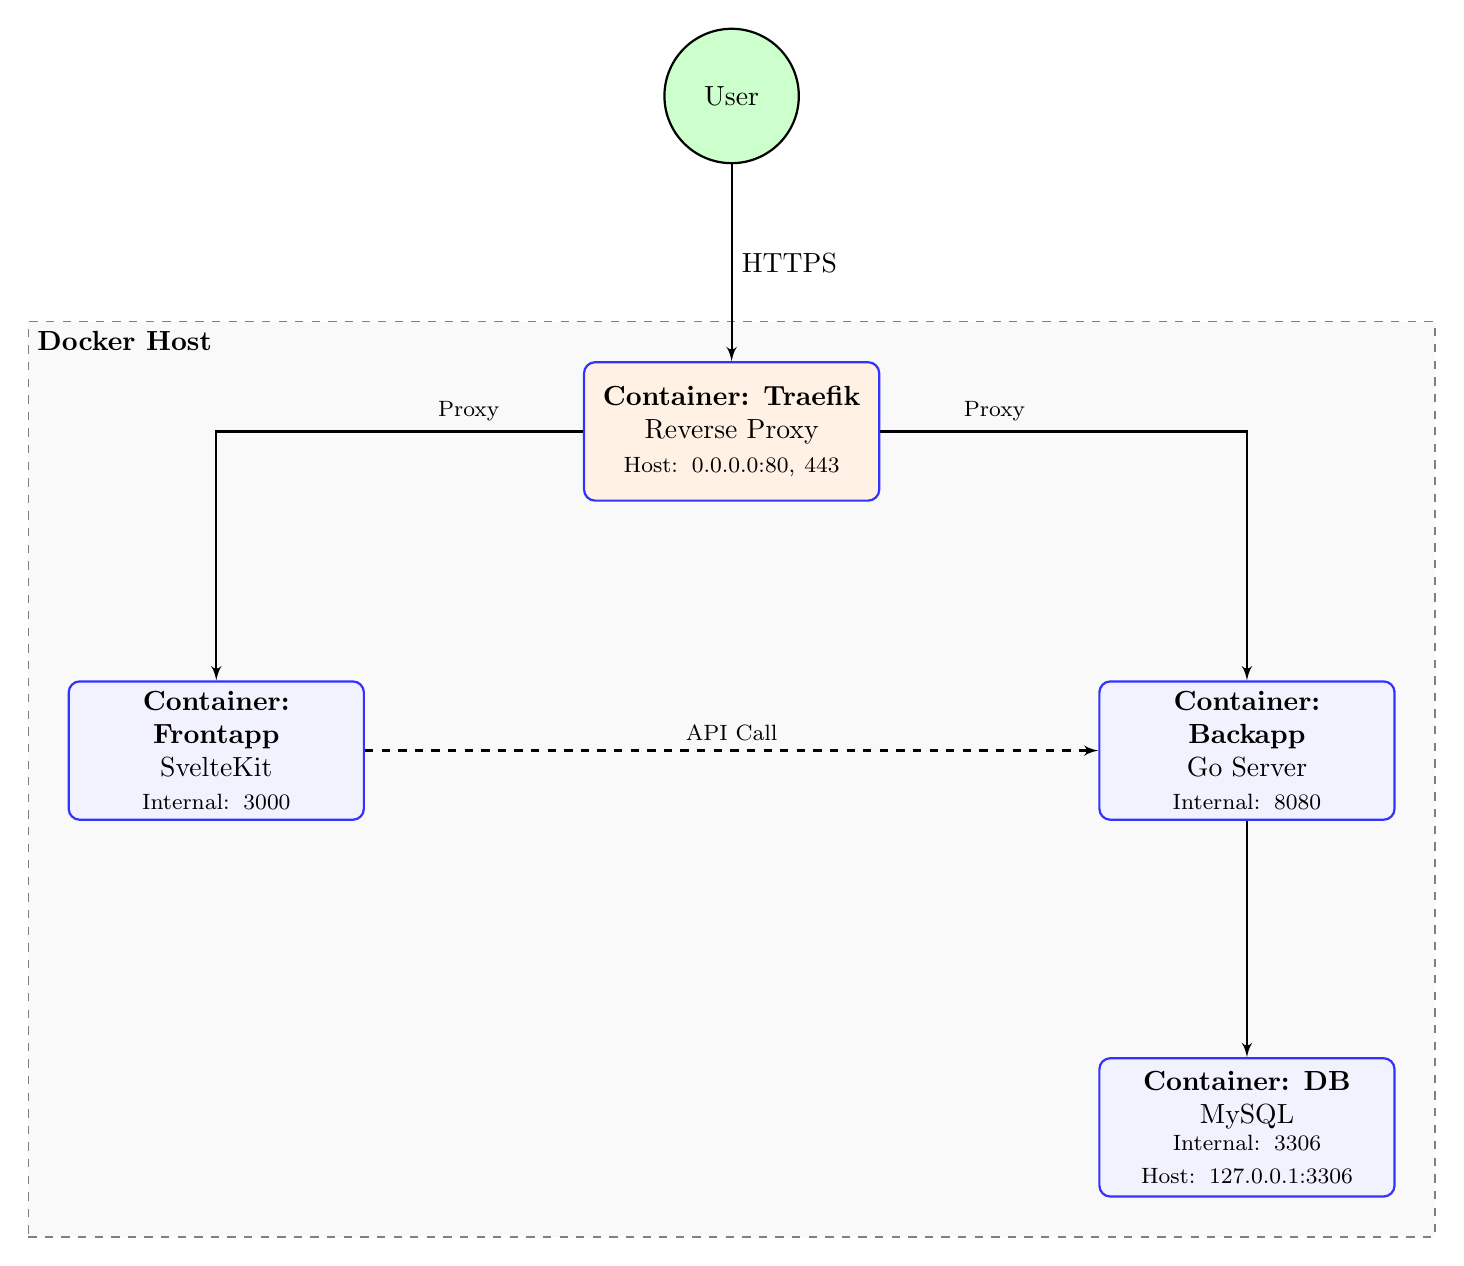
\begin{tikzpicture}[node distance=2.5cm, auto,
            % Styles
            container/.style={rectangle, draw=blue!80, fill=blue!5, thick, text width=10em, text centered, rounded corners, minimum height=5em},
            dbshape/.style={cylinder, cylinder uses custom fill, cylinder body fill=yellow!20, cylinder end fill=yellow!10, shape border rotate=90, aspect=0.25, draw=black, thick, text width=6em, text centered, minimum height=4em},
            user/.style={circle, draw=black, fill=green!20, thick, text width=4em, text centered},
            line/.style={draw, -latex', thick},
            dashedline/.style={draw, -latex', thick, dashed}
        ]

        % Nodes
        \node [user] (user) {User};

        % Traefik
        \node [container, below=of user, fill=orange!10] (traefik) {
            \textbf{Container: Traefik}\\
            Reverse Proxy\\
            \footnotesize{Host: 0.0.0.0:80, 443}
        };

        % Frontend
        \node [container, below left=of traefik, xshift=-1cm, yshift=-0.5cm] (frontend) {
            \textbf{Container: Frontapp}\\
            SvelteKit\\
            \footnotesize{Internal: 3000}
        };

        % Backend
        \node [container, below right=of traefik, xshift=1cm, yshift=-0.5cm] (backend) {
            \textbf{Container: Backapp}\\
            Go Server\\
            \footnotesize{Internal: 8080}
        };

        % Database
        \node [container, below=of backend, yshift=-0.5cm] (db) {
            \textbf{Container: DB}\\
            MySQL\\
            \footnotesize{Internal: 3306}\\
            \footnotesize{Host: 127.0.0.1:3306}
        };

        % Edges
        \path [line] (user) -- node[right] {HTTPS} (traefik);
        \path [line] (traefik) -| node[pos=0.1, above left, font=\footnotesize] {Proxy} (frontend);
        \path [line] (traefik) -| node[pos=0.1, above right, font=\footnotesize] {Proxy} (backend);
        \path [dashedline] (frontend) -- node[above, font=\footnotesize] {API Call} (backend);
        \path [line] (backend) -- (db);

        % Docker Host Box
        \begin{scope}[on background layer]
            \node [draw=black!50, dashed, fill=gray!5, fit=(traefik) (frontend) (backend) (db), inner sep=0.5cm, label={[anchor=north west]north west:\textbf{Docker Host}}] (host) {};
        \end{scope}

    \end{tikzpicture}
    }
    \caption{システム構成図(Dockerコンテナ構成)}
\end{figure}



\end{document}
